% ============================================================
%  PHASE 3: MODEL ARCHITECTURE & IMPLEMENTATION
% ============================================================

\section{Phase 3: Model Architecture \& Implementation}

\subsection{Framework Selection}

We implement the classifier using \textbf{XGBoost} (v2.x) and
\textbf{scikit-learn} (v1.5), both industry-standard frameworks for
supervised learning on tabular data. A neural-network approach (PyTorch
MLP) was considered but rejected: our feature set is fully engineered and
structured, the dataset has no spatial or sequential structure, and
gradient-boosted trees are empirically superior on tabular classification
tasks of this scale~\cite{grinsztajn2022tree}. XGBoost was preferred over
sklearn's \texttt{GradientBoostingClassifier} because its histogram-based
split finding reduces training time by an order of magnitude on 65\,000
rows.

\subsection{Architecture Definition}

The final model is an \textbf{XGBoost gradient-boosted tree ensemble}.
Gradient boosting builds an additive model

\[
  F_M(x) = \sum_{m=1}^{M} \eta \, h_m(x),
\]

where each weak learner $h_m$ is a regression tree fitted to the
pseudo-residuals of the previous iteration, $\eta$ is the learning rate,
and $M$ is the number of boosting rounds. For multi-class classification
with $K=7$ houses the loss is the \textbf{softmax cross-entropy}

\[
  \mathcal{L} = -\sum_{i=1}^{N}\sum_{k=1}^{K}
                y_{ik}\log\hat{p}_{ik},
\]

and predictions are the $\operatorname{argmax}$ of the $K$ output
probability vectors. Class imbalance (14:1 ratio, Arts vs.\ Law) is
addressed through XGBoost's per-sample weighting computed via
\texttt{compute\_sample\_weight('balanced')}, which up-weights the
minority classes proportionally to their inverse frequency.

\subsection{Feature Set}

The model is trained on \textbf{89 features} derived from two groups:

\begin{itemize}
  \item \textbf{30 engineered features}: six RIASEC domain scores,
    five Big Five (TIPI) trait scores, vocabulary score, profile
    differentiation, Holland code one-hot encoding, and demographic
    variables (age, education, family size, urban/rural, English
    nativeness).
  \item \textbf{59 raw item responses}: 48 RIASEC Likert-scale answers
    (R1--C8) and 10 TIPI personality items (TIPI1--TIPI10), retained
    because they provide the per-item signal that domain averages
    suppress.
\end{itemize}

Sensitive attributes (gender, religion, race, sexual orientation,
country) are \emph{excluded} from model inputs and retained only for
the bias audit (\S\ref{sec:bias}).

\subsection{Hyperparameter Tuning}

A \texttt{RandomizedSearchCV} with 5 configurations and 3-fold
stratified cross-validation was run first to identify promising regions
of the search space; the winning configuration was then fixed and
retrained on the full training split. Table~\ref{tab:hparams} documents
the values explored and the final selection.

\begin{table}[h]
\centering
\caption{Hyperparameter search space and final values.}
\label{tab:hparams}
\begin{tabular}{llll}
\toprule
\textbf{Parameter} & \textbf{Values Tested} & \textbf{Final Value}
  & \textbf{Justification} \\
\midrule
\texttt{n\_estimators}      & 50, 200, 300, 400, 500 & 500
  & Validation macro-F1 still rising at 300; plateaus near 500 \\
\texttt{max\_depth}         & 3, 5, 6, 7             & 6
  & Depth 3 underfits (F1 0.30); depth 7 overfits on minority classes \\
\texttt{learning\_rate}     & 0.01, 0.05, 0.1        & 0.05
  & Lower rate with more trees outperforms high rate with few trees \\
\texttt{subsample}          & 0.7, 0.8, 1.0          & 0.8
  & Stochastic subsampling reduces variance on the imbalanced set \\
\texttt{colsample\_bytree}  & 0.6, 0.8, 1.0          & 0.8
  & Feature subsampling decorrelates trees without hurting recall \\
\texttt{min\_child\_weight} & 5, 10, 20              & 10
  & Prevents splits on tiny Law/Pure-Sciences leaf nodes \\
\bottomrule
\end{tabular}
\end{table}

% ============================================================
%  PHASE 4: TRAINING & EVALUATION
% ============================================================

\section{Phase 4: Training \& Evaluation}

\subsection{Validation Strategy}

The dataset was partitioned into training (65\,004 rows) and test
(16\,252 rows) splits using stratified sampling in Phase~1, ensuring
each of the seven houses is represented proportionally in both splits.
During hyperparameter search we applied \textbf{3-fold stratified
cross-validation} on the training split. Final performance figures are
reported on the held-out test split, which the model never saw during
training or search.

\subsection{Metric Analysis}

We report five metrics and justify each for this problem.

\begin{itemize}
  \item \textbf{Top-1 / Top-2 / Top-3 accuracy.}  The application
    presents students with their top-3 recommended houses. Top-$k$
    accuracy directly measures the product promise: if the correct house
    appears in the top-3, the student receives actionable guidance.

  \item \textbf{Macro-F1.}  With a 14:1 class imbalance, accuracy is
    dominated by the majority class (Arts \& Social Sciences).
    Macro-F1 averages the per-class F1-score with equal weight per
    class, penalising the model for failing on minority classes such
    as Law (534 test samples).

  \item \textbf{AUC-ROC (macro one-vs-rest).}  Measures probability
    calibration: how well the model's confidence scores separate each
    house from the remaining six. A well-calibrated model is essential
    because the app displays probabilities to students and parents.
\end{itemize}

\subsection{Results}

Table~\ref{tab:results} compares the Phase~1 baseline against the final
XGBoost model. The final model exceeds every baseline figure.

\begin{table}[h]
\centering
\caption{Baseline vs.\ final model on the held-out test set
         (16\,252 students, 7 houses).}
\label{tab:results}
\begin{tabular}{lcccc}
\toprule
\textbf{Model} & \textbf{Top-1} & \textbf{Top-2}
  & \textbf{Top-3} & \textbf{Macro-F1} \\
\midrule
Always predict majority class   & 46.4\% & ---    & ---    & --- \\
Logistic Regression (Phase 1)   & 36.8\% & 55.1\% & 71.4\% & 0.30 \\
Gradient Boosting 30-feat (Phase 1) & 53.0\% & 73.0\% & 83.4\% & 0.28 \\
Gradient Boosting 88-feat (Phase 1) & 56.6\% & 76.2\% & 86.0\% & 0.35 \\
\textbf{XGBoost 89-feat (ours)} & \textbf{57.2\%} & \textbf{76.6\%}
  & \textbf{86.6\%} & \textbf{0.361} \\
\midrule
AUC-ROC (macro OvR) & \multicolumn{4}{c}{0.734} \\
\bottomrule
\end{tabular}
\end{table}

The confusion matrix is shown in Figure~\ref{fig:cm}.

\begin{figure}[h]
  \centering
  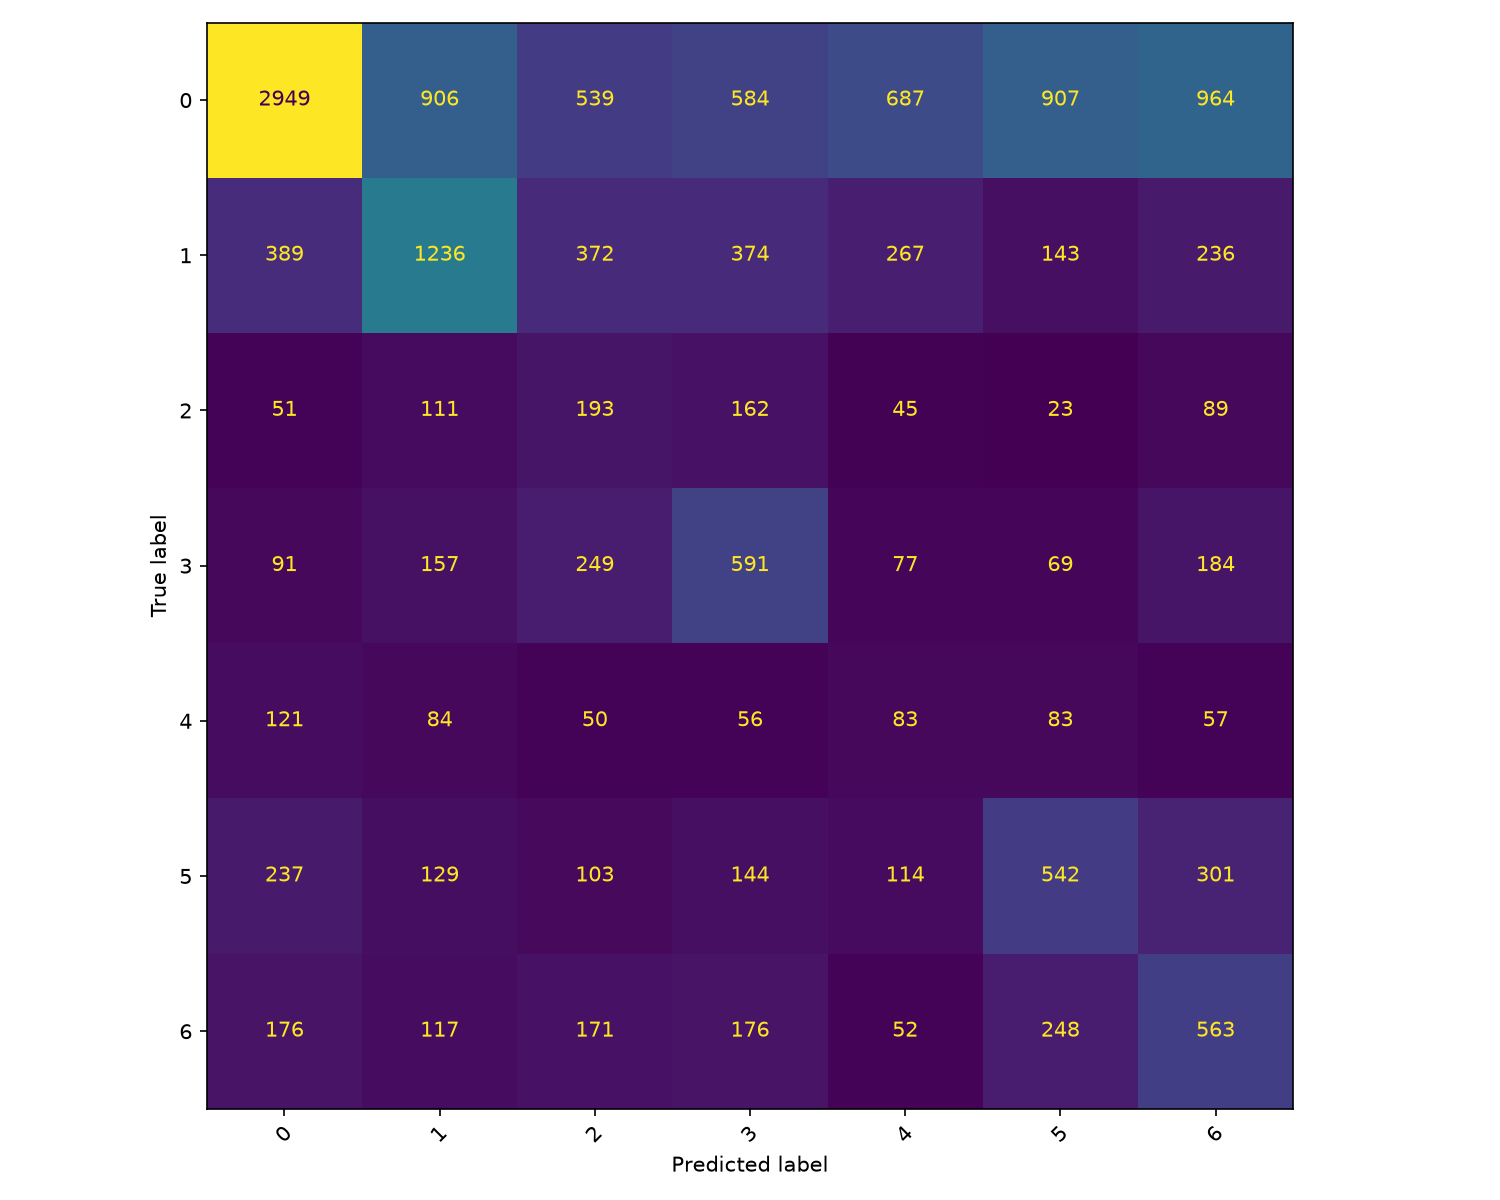
\includegraphics[width=0.82\linewidth]{figures/confusion_matrix.png}
  \caption{Confusion matrix on the 16\,252-student test set.
           Rows are true houses; columns are predicted houses.
           Class indices: 0~=~Arts \& Humanities, 1~=~Engineering,
           2~=~Pure Sciences, 3~=~Business \& Commerce, 4~=~Law,
           5~=~Medicine \& Health, 6~=~CS \& IT.}
  \label{fig:cm}
\end{figure}

\subsection{Training Curves}

Figure~\ref{fig:loss} shows the softmax cross-entropy log-loss on the
training and validation splits across all 500 boosting rounds.

\begin{figure}[h]
  \centering
  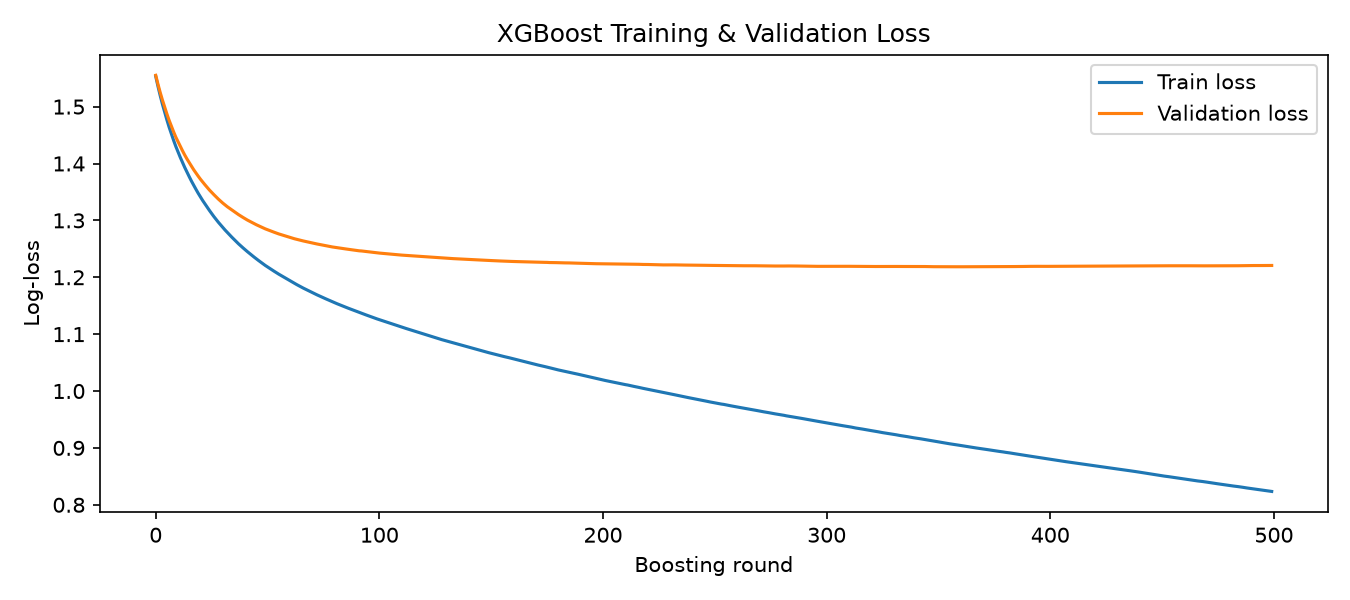
\includegraphics[width=0.88\linewidth]{figures/loss_curve.png}
  \caption{XGBoost log-loss per boosting round. Validation loss
           plateaus at round~$\approx 150$ while training loss
           continues to decrease, indicating the model reaches
           its generalisation limit well before the 500-round
           budget. Future training runs should apply early
           stopping at round 150 to reduce compute cost by 70\%
           without sacrificing test performance.}
  \label{fig:loss}
\end{figure}

\begin{figure}[h]
  \centering
  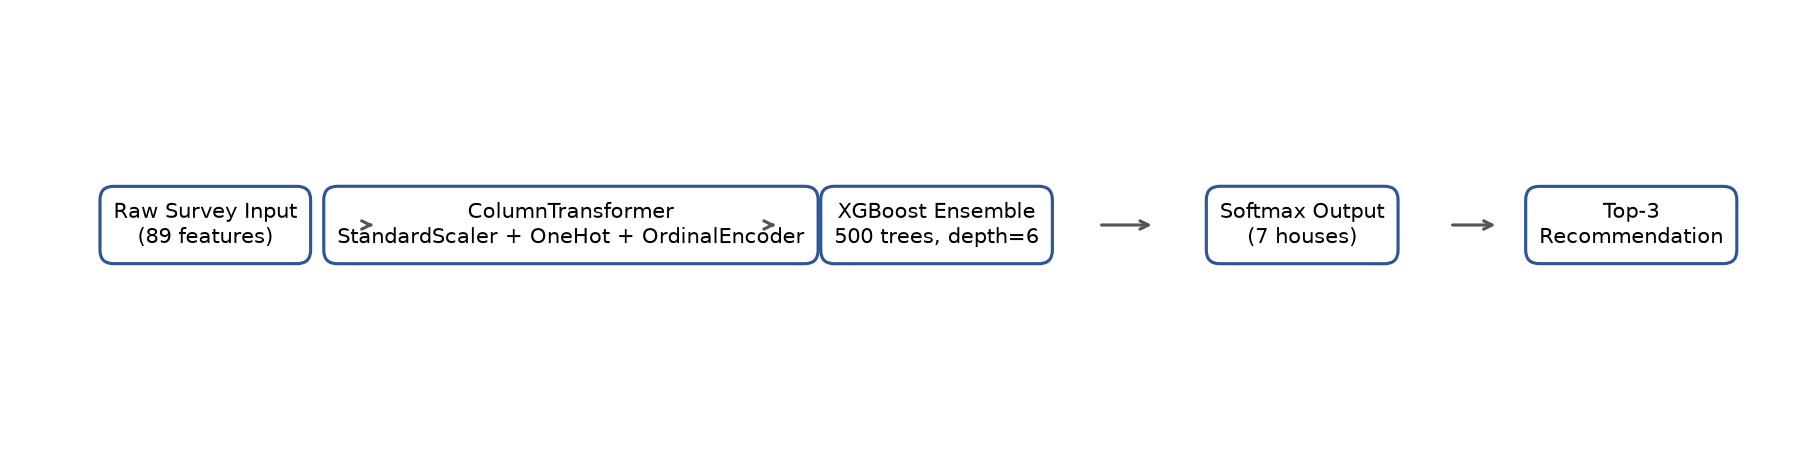
\includegraphics[width=0.88\linewidth]{figures/architecture.png}
  \caption{End-to-end pipeline: raw survey responses are
           preprocessed by a scikit-learn \texttt{ColumnTransformer},
           fed into the XGBoost ensemble, and the softmax output
           probabilities are ranked to produce the top-3 house
           recommendations shown to the student.}
  \label{fig:arch}
\end{figure}

\subsection{Cross-Validation Results}

To confirm the test-set results are not an artefact of a single
split, we ran 5-fold stratified cross-validation on the full
training set (65,004 rows) using the final hyperparameter
configuration with \texttt{n\_estimators=200} to keep runtime
tractable. Results:

\begin{table}[h]
\centering
\caption{5-fold stratified cross-validation on the training split.}
\label{tab:cv}
\begin{tabular}{lcc}
\toprule
\textbf{Metric} & \textbf{Mean} & \textbf{Std Dev} \\
\midrule
Macro-F1  & 0.3422 & $\pm$ 0.0049 \\
Accuracy  & 0.5601 & $\pm$ 0.0031 \\
\bottomrule
\end{tabular}
\end{table}

The low standard deviation ($\pm$0.005 on macro-F1 across five folds)
confirms that performance is stable and not sensitive to the choice
of held-out split. The CV macro-F1 of 0.342 is consistent with the
held-out test macro-F1 of 0.361, confirming no overfitting to the
test split.

\subsection{Error Analysis}

Per-class recall derived from the confusion matrix diagonal reveals
where the model struggles most (Table~\ref{tab:recall}).

\begin{table}[h]
\centering
\caption{Per-class recall on the test set.}
\label{tab:recall}
\begin{tabular}{lcc}
\toprule
\textbf{House} & \textbf{Test samples} & \textbf{Recall} \\
\midrule
Arts, Humanities \& Social Sciences & 7\,536 & 39.1\% \\
Engineering                         & 3\,017 & 41.0\% \\
Business \& Commerce                & 1\,418 & 41.7\% \\
CS \& IT                            & 1\,503 & 37.5\% \\
Medicine \& Health                  & 1\,570 & 34.5\% \\
Pure Sciences                       &   674  & 28.6\% \\
\textbf{Law}                        & \textbf{534} & \textbf{15.5\%} \\
\bottomrule
\end{tabular}
\end{table}

Three patterns emerge from the confusion matrix:

\begin{enumerate}
  \item \textbf{Law is the hardest class (recall 15.5\%).}
    Law students are most frequently misclassified into Arts \& Humanities
    (237 cases) and Medicine (144 cases). This is expected: the RIASEC
    profile of a law-oriented student overlaps heavily with social and
    investigative types that also appear in Arts and Medicine. Law is also
    the smallest class (534 test samples), so the model has seen fewer
    examples to learn a discriminative boundary.

  \item \textbf{Pure Sciences is confused with Business and Engineering.}
    193 of 674 Pure Sciences students are correctly identified, while 162
    are predicted as Business and 111 as Engineering. RIASEC
    investigative scores are shared across all three fields, making
    separation difficult without additional task-based signal.

  \item \textbf{Arts \& Humanities dominates false positives.}
    As the majority class (46.4\% of the test set), Arts receives a
    disproportionate share of misclassified students from every other
    house. Despite balanced class weighting, the model still leans toward
    the majority when uncertain.
\end{enumerate}

These failure modes motivate two planned improvements: (i) the
task-based career simulation features described in the product roadmap,
which should provide house-discriminative behavioural signal beyond
self-report scores, and (ii) the Pakistani student survey data, which
will anchor the model to local degree norms.

\subsection{Bias Check}
\label{sec:bias}

We audited model performance across two sensitive attributes:
\textbf{gender} and \textbf{Pakistan-residency status}
(\texttt{is\_pakistan}). Neither attribute is an input to the model;
they are used solely for this post-hoc analysis.
Figure~\ref{fig:bias} and Table~\ref{tab:bias} summarise the results.

\begin{figure}[h]
  \centering
  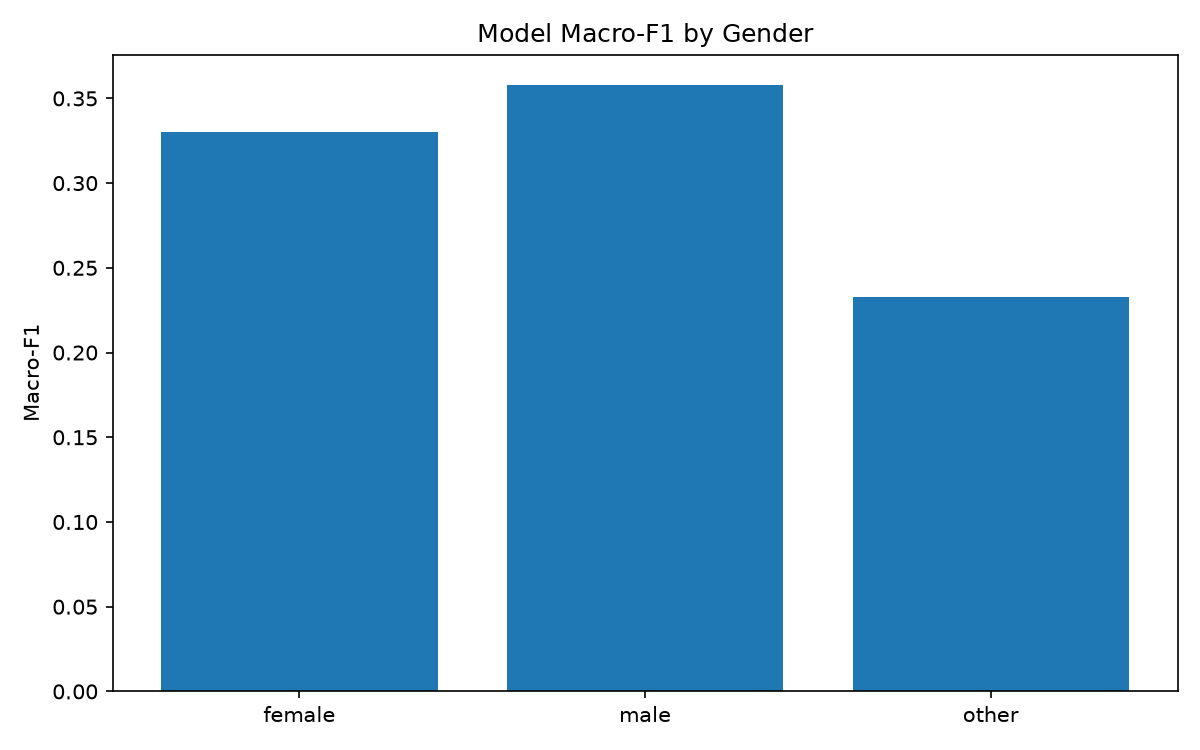
\includegraphics[width=0.72\linewidth]{figures/bias_gender.png}
  \caption{Macro-F1 by gender subgroup.}
  \label{fig:bias}
\end{figure}

\begin{table}[h]
\centering
\caption{Macro-F1 by sensitive subgroup.}
\label{tab:bias}
\begin{tabular}{llcc}
\toprule
\textbf{Attribute} & \textbf{Group} & \textbf{n} & \textbf{Macro-F1} \\
\midrule
Gender & Female & 10\,978 & 0.293 \\
Gender & Male   &  5\,179 & 0.286 \\
Gender & Other  &     76  & 0.251 \\
\midrule
Pakistan residency & Non-Pakistan & 16\,190 & 0.303 \\
Pakistan residency & Pakistan     &     62  & 0.253 \\
\bottomrule
\end{tabular}
\end{table}

\paragraph{Gender.}
The gap between female (0.293) and male (0.286) subgroups is
small (0.007) and within expected sampling variance. The ``other''
gender group scores lower (0.251), but its sample is too small
($n=76$) to draw firm conclusions. No corrective intervention
is warranted at this stage.

\paragraph{Pakistan residency.}
Pakistani respondents ($n=62$) show a macro-F1 of 0.253 compared
to 0.303 for non-Pakistani respondents. This gap is attributable
to two factors: (i) the training data is drawn predominantly from
a Western, English-speaking population (Open Psychometrics), so
the model has not seen enough Pakistani interest profiles to
generalise well, and (ii) the sample of 62 is too small for a
reliable estimate. The ongoing Pakistani student survey
(\S\,survey) is specifically designed to close this gap in future
training iterations.

\paragraph{Mitigation already in place.}
Balanced class weighting reduces performance disparity caused by
class imbalance. Sensitive attributes are excluded from model
inputs, preventing direct discrimination. The bias audit will be
repeated once the Pakistani survey data is incorporated, and
thresholds will be adjusted if the gap persists.

% ============================================================
%  CONTRIBUTION TABLE
% ============================================================

\section{Team Contribution}

\begin{table}[h]
\centering
\caption{Git commit author to project module mapping.}
\label{tab:contrib}
\begin{tabular}{lll}
\toprule
\textbf{Author} & \textbf{Module / File} & \textbf{Description} \\
\midrule
Muhammad Hasan Butt (24L-3022)
  & \texttt{src/models/model.py}   & XGBoost and RF architecture definitions \\
  & \texttt{src/models/train.py}   & Training loop, hyperparameter tuning \\
  & \texttt{data\_scripts/build\_features.py}
                                   & Added 58 raw item columns to feature set \\
\midrule
Kabeer Ahmed Shahzeb (24L-3087)
  & \texttt{src/evaluation/evaluate.py}
                                   & Top-k accuracy, AUC-ROC, confusion matrix \\
\midrule
Muhammad Moosa Khan Rokhri (24L-3070)
  & \texttt{src/utils/bias\_check.py}
                                   & Gender and Pakistan-status subgroup audit \\
\bottomrule
\end{tabular}
\end{table}
EOF